% TEX INPUTS=.:$HOME/git/bvtex: latexmk  -pdf <main>.tex
\documentclass[xcolor=dvipsnames]{beamer}
\usefonttheme{serif}

\input{defaults}
\input{beamer/preamble}
\usepackage{svg}
\usepackage{wasysym}


\setbeamertemplate{navigation symbols}{}
% \setbeamertemplate{background}[grid][step=1cm]

\usepackage{siunitx}
\usepackage{xmpmulti}
\usepackage[export]{adjustbox}
\usepackage{ulem}
\usepackage[outline]{contour}
\usepackage{pdfpages}
\usepackage{tikz}
\usetikzlibrary{shapes.geometric, arrows}
\usetikzlibrary{positioning}

\definecolor{bvtitlecolor}{rgb}{0.98, 0.92, 0.84}
\definecolor{bvoutline}{rgb}{0.1, 0.1, 0.1}

\renewcommand{\bvtitleauthor}{Brett Viren}
\renewcommand{\bvtit}{WCT Imaging Status}
\renewcommand{\bvtitle}{\LARGE TITLE}
\renewcommand{\bvevent}{{\small EVENT -- DATE}}
\renewcommand{\bvdate}{22 Mar 2019}
\renewcommand{\bvbeamerbackground}{}

\def\Put(#1,#2)#3{\leavevmode\makebox(0,0){\put(#1,#2){#3}}}

\begin{document}
\begin{frame}
  \begin{center}
    \huge
    Progress adding 3D imaging to

    the Wire-Cell Toolkit
  \end{center}
\end{frame}

\begin{frame}
  \frametitle{Process}
  \begin{columns}
    \begin{column}{0.5\textwidth}
      \begin{itemize}
      \item Follow Xin's  \href{https://www.phy.bnl.gov/~bviren/tmp/wctimg/integration_imaging.pptx}{WCP imaging summary slides}
      \item Follow Xin's high level ``imaging flow'' $\rightarrow$
      \item Stare at WCP code, but no copy-paste allowed! \smiley{}
      \item Add some new ideas and optimizations.
      \item Development steps:
        \begin{enumerate}\scriptsize
        \item implement basic operations as ``util'' code.
        \item Design WCT data and component interfaces.
        \item Iterate as realism is added (ie, test on full sim/data, dead wire support).
        \end{enumerate}
      \end{itemize}
    \end{column}
    \begin{column}{0.5\textwidth}
      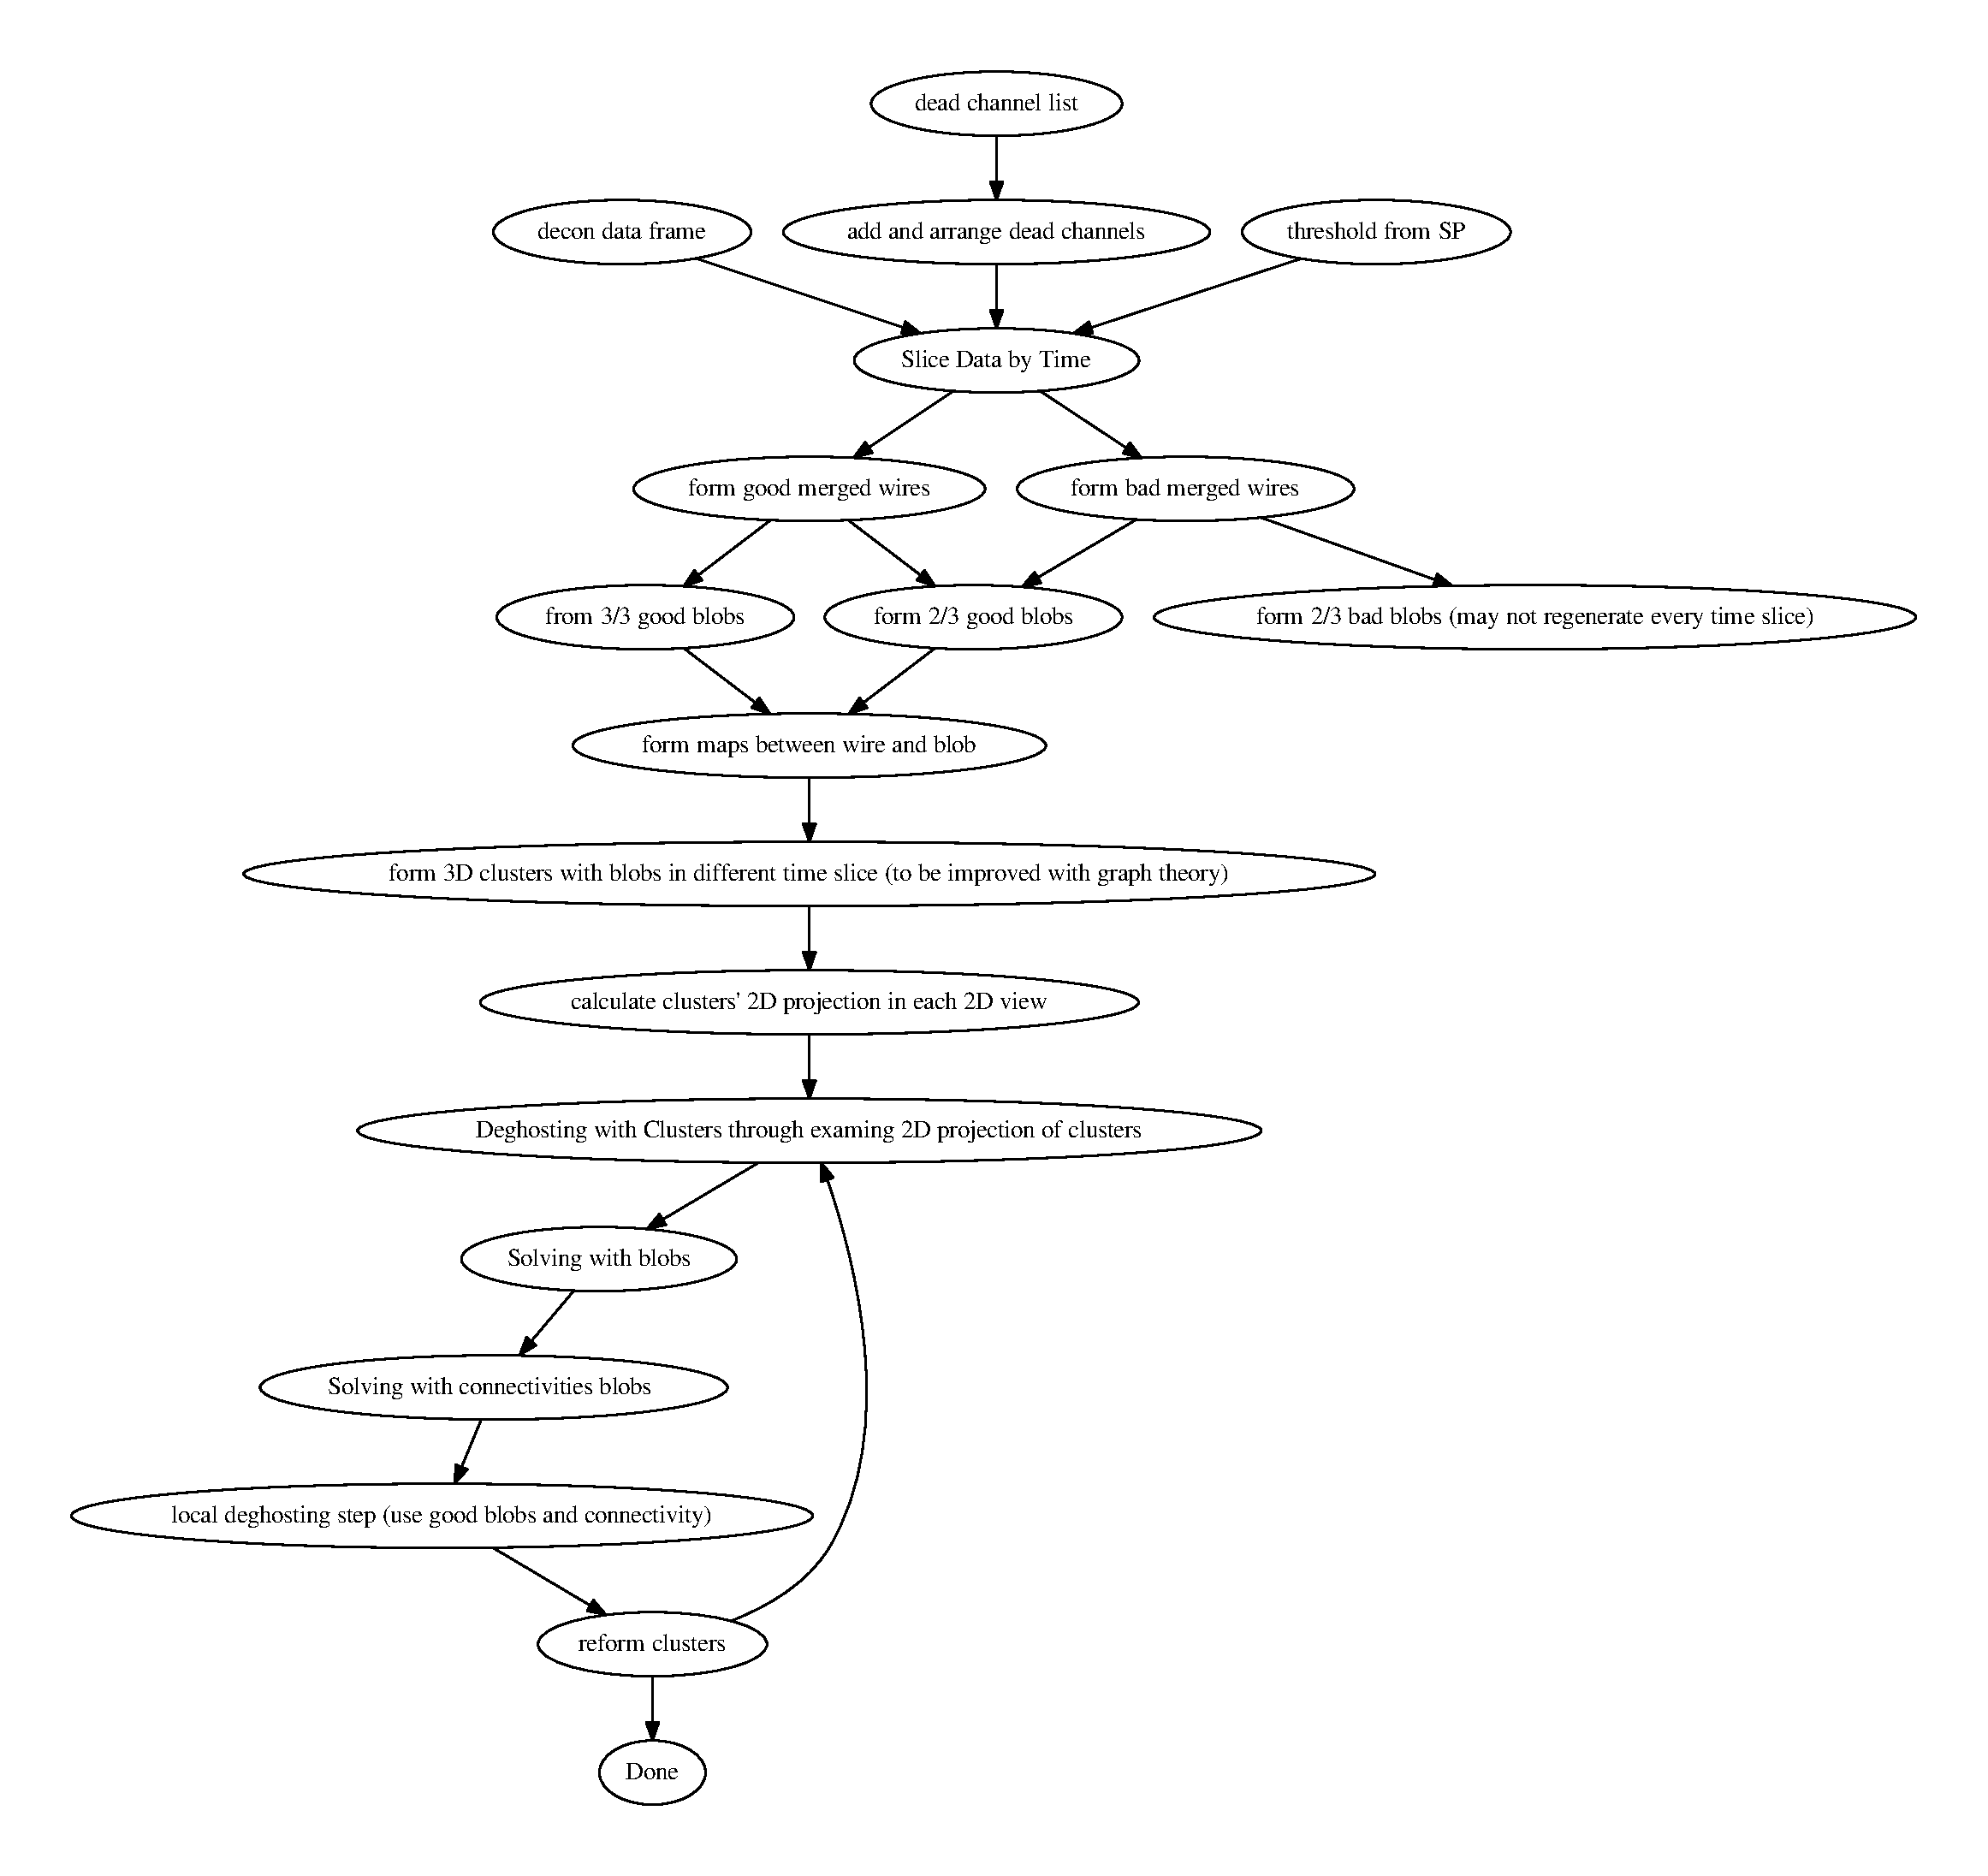
\includegraphics[width=1.1\textwidth]{imaging_flow.pdf}
    \end{column}
  \end{columns}
\end{frame}

\begin{frame}
  \frametitle{Core, high level operations}
  \begin{itemize}
  \item Slicing (done)
  \item Striping (done, but in the end, not needed)
  \item Tiling (done)
  \item Clustering (done)
  \item Solving (in progress)
  \end{itemize}
  \vfill
  ``done'', here, means code works on idealized tests.
  \vfill
  I'll next go through each one.
\end{frame}

\begin{frame}
  \frametitle{Slicing}
  \begin{quote}
    Cut up a readout \textbf{frame} of signals into a queue of time \textbf{slices} with each slice holding a set of \textbf{active channels} and the sum of their waveform sample values in the time \textbf{span} of the slice.
  \end{quote}


  \begin{itemize}
  \item A \textbf{slice} data object has:
    \begin{description}
    \item[ident] some identifying \textbf{number}
    \item[start] when in \textbf{time} the slice begins.
    \item[span] the \textbf{duration} of the time interval covered.
    \item[activity] a \textbf{map} from channel to a value (signal charge)
    \item[frame] a back-pointer to the original \textbf{frame}. 
    \end{description}
  \item Algorithm: the obvious thing.
  \end{itemize}
\end{frame}

\begin{frame}
  \frametitle{Striping}

  \begin{quote}
    Collect all  \textbf{channels} in a \textbf{slice} with a \textbf{value} above a \textbf{threshold} along with their \textbf{connected wires} such that the wires are \textbf{contiguous} in their plane.
  \end{quote}

  \begin{itemize}
  \item In DUNE a stripe may ``wrap'' around the APA, both in terms of the wire conductors and the list of channels.
  \item In the end, this wasn't needed for \textbf{tiling} (next).
  \item However, it has a ``cute'' solution:
  \end{itemize}
  \begin{enumerate}\footnotesize
  \item Build a \textbf{graph} with each \textbf{channel} above threshold connected to its 1, 2 or 3 \textbf{wires} and in that set connect each wire to its \textbf{neighbor} in the plane.
  \item Call \texttt{boost::connected\_components()}, done!
  \end{enumerate}
  The returned value is effectively the list of ``stripes'' for the slice.
\end{frame}

\begin{frame}
  \frametitle{Tiling}

  \begin{quote}
    Tiling identifies \textbf{spatial regions in a slice} which are \textbf{likely consistent} with containing \textbf{ionization activity} based on knowing \textbf{wire geometry} and \textbf{channels above threshold}.
  \end{quote}
  \begin{itemize}\footnotesize
  \item   Although, more accurately we \textbf{remove} regions which are \textbf{definitely not consistent} with....

  \item Tiling is the core starting point for 3D imaging, and inherently very \textbf{combinatoric} so optimizations are very welcome.

  \item And a nice one has been found....

  \end{itemize}
\end{frame}

\begin{frame}
  \frametitle{Ray Grid Optimization}

  \begin{quote}
    Exploit \textbf{uniform wire angle and pitch} to make wire geometry calculations cheap.
  \end{quote}
  

  The concepts are actually rather simple but they need some detailed slides....


\end{frame}

\begin{frame}
  \frametitle{Ray Grid}

  \textbf{Ray}: (as used here) is a \textbf{line segment} defined by \textbf{two 3D endpoints} and a \textbf{direction}.    

  \begin{itemize}
  \item Each real wire (segment) has an associated ray.
  \item Define two parallel rays, \textbf{ray0} and \textbf{ray1} offset by $\pm\frac{1}{2}$ pitch on each side of \textbf{wire 0} for each wire plane.

  \item This ray pair may define a 2D coordinate system:
    \begin{itemize}\footnotesize
    \item[$\circ$] origin: center of \textbf{ray0} (projected to $x=0$)
    \item[$\to$] $\hat{z}$ axis along $\overrightarrow{pitch}$
    \item[$\uparrow$] $\hat{y}$ axis along $\overrightarrow{ray}$
    \item[$\otimes$] $\hat{x}$ by RHR (anti-drift direction)
    \end{itemize}
  \item[$\leftrightarrow$] Also defines a \textbf{1-D linear grid} along plane pitch direction.    
  \item[$\Rightarrow$] Specifying a \textbf{ray index} specifies a \textbf{pitch location}.
  \item[$\Rightarrow$] Valid \textbf{ray indices} $\in[0...N_{wires}]$ (inclusive and for each plane)
  \end{itemize}
  Thus, each \sout{wire plane} \textbf{layer} has a \textbf{ray grid}.

  \tiny I'll say why I change names to ``layer'' in a bit.

\end{frame}

\begin{frame}
  \frametitle{3-layer example of Ray Grid vectors}
  \begin{center}
    \tiny
    \includesvg[height=0.8\textheight]{test_raytiling-00}

    \footnotesize
    \textbf{ray0}/\textbf{ray1} pairs for \textcolor{red}{\textbf{U}},\textcolor{blue}{\textbf{V}},\textbf{W} planes.
    Other vectors described next.

  \end{center}
\end{frame}

\begin{frame}
  \frametitle{Two Ray Grids}
  
  \begin{quote}
    Combining two 1-D ray grids form a \textbf{regular 2D grid}, may provide a \textbf{non-orthogonal coordinate system}.     
  \end{quote}

  Each ray grid is one ``layer''.
  \begin{description}
  \item[$p^l$] relative \textbf{pitch vector} for layer $l$.
  \item[$c^l$] the \textbf{origin point} (center of \textbf{ray0}) for layer $l$.
  \item[$r^{lm}_{ij}$] a \textbf{crossing point} of ray $i$ from layer $l$ \\
    and ray $j$ from layer $m$.
  \item[$w^{lm}$] relative \textbf{displacement vector} for layer $l$ connecting crossing points of neighboring layer-$m$ rays on a ray of layer $l$.
  \end{description}
  \begin{center}
    \footnotesize
    (revisit diagram on previous slide)
  \end{center}
\end{frame}

\begin{frame}
  \frametitle{The Key Optimization}
  Given vectors $p^l$, $c^l$ and tensor $w^{lm}$ for \textbf{two layers} and one explicitly calculated crossing point $r^{lm}_{00}$ the tensor of \textbf{all other crossing points} $r^{lm}_{ij}$ is trivial:
  \vspace{-5mm}
  \begin{center}
    \[r^{lm}_{ij} = r^{lm}_{00} + j w^{lm} + i w^{ml}\]
  \end{center}

  \begin{itemize}
  \item $r^{lm}_{00}$ and $w^{lm}$ can be calculated with simple vector arithmetic
  \item \textbf{For $N$ layers}: must calculate for \textbf{every pair of layers}.
    \begin{itemize}
    \item[$\circ$] This is $\mathcal{O}(\frac{1}{2}N^2)$ but $N=5$ so we don't care.
      \begin{itemize}\scriptsize
      \item[?]  (why 5 and not 3?  it's coming!)

      \end{itemize}
    \end{itemize}
  \end{itemize}
\end{frame}


\begin{frame}
  \frametitle{2-Layer crossing points in a $3^{rd}$ layer}
  \begin{quote}
    Core tiling operation: given a \textbf{crossing point} $r^{lm}_{ij}$ what is its \textbf{pitch location} in a $3^{rd}$, layer $n \not\in\{l,m\}$.
  \end{quote}
  The tensor $P$ of all such pitch locations:
  \vspace{-5mm}
  \begin{center}
    \[P^{lmn}_{ij} = (r^{lm}_{ij} - c^n) \cdot \hat{p}^n\]
  \end{center}

  Where $\hat{p}^n$ is unit vector in pitch direction of layer $n$.\\
  Expanding $r^{lm}_{ij}$ from last slide, 
  \vspace{-5mm}
  \begin{center}
    \[P^{lmn}_{ij} = r^{lm}_{00}\cdot \hat{p}^n + jw^{lm} \cdot \hat{p}^n + iw^{ml} \cdot \hat{p}^n - c^n \cdot \hat{p}^n\]
  \end{center}
  Or more simply,
  \vspace{-5mm}
  \begin{center}
    \[P^{lmn}_{ij} = ja^{lmn} + ia^{mln} + b^{lmn},\ (l \ne m \ne n)\]
  \end{center}
The tensors $a$ and $b$ are scalar valued, $a$ is not symmetric under a transpose of $l$ and $m$ and $b$ is.  Both have undefined diagonals

\end{frame}

\begin{frame}
  \frametitle{Crossing point containment}
  Okay, the operation that is \textbf{really} needed is:\footnote{In WCP language: ``is a \textit{blob corner} in a \textit{merged wire}?''}

  \begin{quote}
    What rays in layer $n$ bound a given crossing point $r^{lm}_{ij}$ of layers $l$ and $m$?
  \end{quote}

  We simply normalize $P^{lmn}_{ij}$ by the pitch and truncate to get the \textbf{index of the ray} which is \textbf{at or just below} (in pitch) the \textbf{crossing point}:

  \vspace{-5mm}
  \begin{center}
    \[I^{lmn}_{ij} \equiv floor(P^{lmn}_{ij}/p^n)\]
    \[(l \ne m \ne n)\]
  \end{center}
\end{frame}

\begin{frame}
  \frametitle{Ray Grid Optimization Summary}
  We can now \textbf{very quickly} find:

  \begin{itemize}
  \item any crossing point of two rays (in different ray grids),
  \item the pitch location in a $3^{rd}$ layer of this crossing point,
  \item the index of the nearby ray and thus
  \item the corresponding wire and the corresponding channel.
  \end{itemize}

  \begin{center}
    These are the building blocks.  Now, on to tiling....    
  \end{center}

\end{frame}

\begin{frame}
  \frametitle{Tiling prelude: Activity and why 5 layers}

  \begin{quote}
    \textbf{Activity array}: a 1-D array, defined on a \textbf{ray grid}, with elements indicating possible ``activity'' somewhere near the ray\footnote{Each element is a ``fired wire'' in WCP language}.
  \end{quote}

  \begin{itemize}
  \item Gives $\mathcal{O}(1)$ lookup of a wire/channel given a pitch.
  \item   For each plane, U, V and W the \textbf{activity array} is simply the channel \textbf{charge values} in the time slice \textbf{ordered/limited} by the \textbf{wires in the plane}.

  \item Add to these, \textbf{two special layers}, each of a single ``wire'' and ``channel'' which are \textbf{always active} and with a ``pitch'' equal to the height or width, respectively, of the sensitive area of the anode.

  \end{itemize}

  Tiling  thus solves a $2+N$ layer problem where $N = 3$ for pD/DUNE/MB but can be naturally extended to $N=4+$.

\end{frame}


\begin{frame}
  \frametitle{Activity arrays illustrated with toy simulation}
  \begin{columns}
    \begin{column}{0.35\textwidth}
      \footnotesize
      \begin{itemize}
      \item Make random clusters of ``electrons'' in one slice.
      \item For each, find nearest wire from each plane and assign it +1 hit.
      \item Channels sum all hits on attached wires.
      \item Non-zero activity array elements colored by their plane.\\(threshold: $n_{hit}>0$)
      \item The 2 special horiz/vert boundary layers are in gray.
      \end{itemize}
    \end{column}

    \begin{column}{0.7\textwidth}
      
      \begin{center}
        \tiny
        \includesvg[height=0.8\textheight]{test_raytiling-01.svg}
      \end{center}
    \end{column}

  \end{columns}
\end{frame}

\begin{frame}
  \frametitle{Activity array to Strips}
  \begin{columns}
    \begin{column}{0.35\textwidth}
      \footnotesize
      \begin{itemize}
      \item Scan each activity array to find contiguous regions above threshold.
      \item Collect set  $\{s_{ii'}^l\}$ of strips in layer $l$ bound by ray~$i$ and ray~$i'$.
      \end{itemize}
      
    \end{column}

    \begin{column}{0.7\textwidth}

      \begin{center}
        \tiny
        \includesvg[height=0.8\textheight]{test_raytiling-02.svg}
      \end{center}
    \end{column}

  \end{columns}
\end{frame}

\begin{frame}
  \frametitle{Strips to Blobs}
  \begin{quote}
    Blob: a contiguous region of mutual intersections of strips from all layers.
  \end{quote}
  Procedure (ignoring some optimizations):

  \begin{enumerate}
  \item Given layers $0,1$: find set of all crossing points $\{r_{ij}^{01}\}$ of the \textbf{strip boundary rays} from $\{S_{ii'}^l\},\ l \in{0,1}$.
  \item Add layer 2: find set $\{r_{ij}^{l2}, r_{ij}^{2l}\}$ for $l \in {0,1}$
  \item Discard any crossing point $\{r_{ij}^{lm}\}$ which is not in a strip of any other layer $n \not\in \{l,m\}$.
  \item \texttt{goto} 2 for layers 3, 4, 5, ....
  \end{enumerate}

  \begin{itemize}
  \item This is the \textbf{inherently combinatoric} process.
    \begin{itemize}\footnotesize
    \item[$\circ$] good thing ray grid optimization is so fast!
    \end{itemize}
  \end{itemize}

  Next, I walk through an example applying each layer to the toy simulation....
\end{frame}

\begin{frame}
  \frametitle{Layers 0, 1}
  \begin{columns}
    \begin{column}{0.35\textwidth}
      \footnotesize
      \begin{itemize}
      \item L0+L1 is trivial.
      \item A single blob results which spans the  overlap of the single horizontal and vertical strips and thus exactly spans the active area of the anode.
      \item The example detector is $100\times100$ distance units in size.
      \end{itemize}
      
    \end{column}

    \begin{column}{0.7\textwidth}

      \begin{center}
        \tiny
        \includesvg[height=0.8\textheight]{test_raytiling-04.svg}
      \end{center}
    \end{column}

  \end{columns}
\end{frame}

\begin{frame}
  \frametitle{Layers 0, 1, 2}
  \begin{columns}
    \begin{column}{0.35\textwidth}
      \footnotesize
      \begin{itemize}
      \item L0+L1+L2 adds first actual wire plane
      \item The previous single blob is broken into three.
      \item Each blob is defined by a pair of boundary rays from each layer.
      \end{itemize}
      
    \end{column}

    \begin{column}{0.7\textwidth}

      \begin{center}
        \tiny
        \includesvg[height=0.8\textheight]{test_raytiling-05.svg}
      \end{center}
    \end{column}

  \end{columns}
\end{frame}

\begin{frame}
  \frametitle{Layers 0, 1, 2, 3}
  \begin{columns}
    \begin{column}{0.35\textwidth}
      \footnotesize
      \begin{itemize}
      \item L0+L1+L2+L3 adds second wire plane
      \item Three blobs become eight.
      \item Knowing the ``true electrons'' we start to see ghosts.
      \end{itemize}
      
    \end{column}

    \begin{column}{0.7\textwidth}

      \begin{center}
        \tiny
        \includesvg[height=0.8\textheight]{test_raytiling-06.svg}
      \end{center}
    \end{column}

  \end{columns}
\end{frame}

\begin{frame}
  \frametitle{Layers 0, 1, 2, 3, 4}
  \begin{columns}
    \begin{column}{0.35\textwidth}
      \footnotesize
      \begin{itemize}
      \item L0+L1+L2+L3+L4 adds final wire plane
      \item Eight blobs become 13.
      \item Some ghosts reduced in size and increased in number. 
      \item Some ghosts may be removed, but not in this example.
      \end{itemize}
      
    \end{column}

    \begin{column}{0.7\textwidth}

      \begin{center}
        \tiny
        \includesvg[height=0.8\textheight]{test_raytiling-07.svg}
      \end{center}
    \end{column}

  \end{columns}
\end{frame}

\begin{frame}
  \frametitle{Final result + original strips}
  \begin{columns}
    \begin{column}{0.35\textwidth}
      \footnotesize
      
    \end{column}

    \begin{column}{0.7\textwidth}

      \begin{center}
        \tiny
        \includesvg[height=0.8\textheight]{test_raytiling-08.svg}
      \end{center}
    \end{column}

  \end{columns}
\end{frame}



\begin{frame}
  \frametitle{Clustering}
  \begin{quote}
    Clustering (here) is the \textbf{association} of blobs between neighboring time slices based on their relative positions.
  \end{quote}
  \begin{itemize}
  \item Essentially an extension of tiling except compare blob corners (still ray grid crossing points) in one slice against strip bounds of blobs in another slice.
  \item Can be used for applying \textbf{connectivity conditions} to remove some ghosts, in ``solving'' or to build extended 3D clusters.
  \item Currently, the definition of ``overlap'' of blobs is hard-wired.  This can be improved to allow some parameterized ``overlap distance'' to be used. 
  \end{itemize}
\end{frame}

\begin{frame}[fragile]
  \frametitle{Clustering visitor}
  Clustering is a generic function which takes two lists of blobs and a \textbf{functor}:
\begin{verbatim}
    auto assoc = some_function_object;
    RayGrid::associate(blobs_1, blobs_2, assoc);
\end{verbatim}

  The \texttt{associate()} function will call the \texttt{assoc} functor for every pair of blobs which are associated.

  \vfill

  It's then up to the user to do something fun in their functor.
\end{frame}

\begin{frame}
  \frametitle{Visualization}
  \begin{columns}
    \begin{column}{0.35\textwidth}
      \footnotesize
      
    \begin{itemize}
    \item Support writing VTK files for ParaView and MayaVi.
    \item A little ``hacky'' but good for debugging.
    \item Shows blobs resolved from two line sources crossing at a point.
    \item Each ``plate'' is one blob.  
    \item Color represents slice number.
    \end{itemize}

    \end{column}
    \begin{column}{0.7\textwidth}

      \begin{center}
        \tiny
        \includesvg[height=0.8\textheight]{x.svg}    
      \end{center}
    \end{column}

  \end{columns}
\end{frame}

\begin{frame}
  \frametitle{Solving}
  \begin{quote}
    Use measured charge information and wire geometry to invert $M=G\cdot S$.
  \end{quote}
  $S$ is charge in each blob, $G$ is blob-channel connection, $M$ is measured charge in channels.
  \begin{itemize}
  \item This work is just starting.
  \item It brings together blobs built from both APA faces because \textbf{now} wrapping adds complication.
  \item Maybe use connected subgraph trick (see ``striping'') to partition $G$ into smaller problems?
  \item Maybe look for an alternative to \texttt{ress}? 
    Or, is it already the best available?
  \end{itemize}

\end{frame}

\begin{frame}
  \frametitle{Yet More To Do}
  \begin{itemize}
  \item Complete the solving stage.
  \item Configure full chain test starting with trivial line sources.
  \item One more pass through my thinking to see how/where to handle dead channels.
  \item Test on real sim and real data.
  \item Help others to use, improve and validate.
  \end{itemize}

  A lot of more work, but progress is getting made!
\end{frame}

\end{document}

